\documentclass[professionalfonts, xcolor={usenames,svgnames,x11names,table}]{beamer}

\usetheme{SBUclass}
\usepackage{mypackages}
\usepackage{mycommands}


\title{\texorpdfstring{Language \& Technology}{Language and Technology}}
\subtitle{Lecture 6: String Matching}
\author{Al{\"e}na Aks{\"e}nova \& Aniello De Santo}
\institute{Stony Brook University\\\texttt{alena.aksenova@stonybrook.edu}\\\texttt{aniello.desanto@stonybrook.edu}}
\date{}

\begin{document}
\unnumbered{
\begin{frame}
	\titlepage
\end{frame}
}

\begin{frame}{I had a Very Fun Saturday\ldots}
    \begin{itemize}
        \item \textbf{Task:}\\
            collect data on SBC-certified courses over last 5 years
        \item \textbf{Solution:}
            \begin{itemize}
                \item Download all archived undergraduate bulletins.
                \item For each course, extract which SBC requirements it satisfies.
            \end{itemize}
    \end{itemize}

    \pause
    \begin{block}{But how do you do that?}
        \begin{itemize}
            \item $\approx$3,500 registered courses 
            \item course descriptions scattered across 140 files per semester
            \item For a 5-year period, that's over \highlight{35,000} course descriptions scattered over \highlight{1,400 files}!
        \end{itemize}
    \end{block}
\end{frame}

\begin{frame}[fragile]{The Final Solution}
    \begin{itemize}
        \item This took quite a bit of data massaging with Python.
        \item But the central step is condensing course descriptions into\\
            a list of the form
    \end{itemize}
\begin{pythoncode}
    [program, course_number, course_name, SBCs]
\end{pythoncode}
    \pause
    \begin{itemize}
        \item And here is the central piece of code that does the trick:
    \end{itemize}
\begin{pythoncode}
    re.sub(r'^.*?id="(\w+)".*?<h3>.*?:\s*(.*?)</h3>.*?<p>(.*?)</p>(.*)',
           r"\1|\2|\3|\4",
           course_description)
\end{pythoncode}
    \pause
    \begin{itemize}
        \item What the heck is that? It's the miraculous\\
            (and highly illegible) world of \highlight{regular expressions}!
    \end{itemize}
\end{frame}

\begin{frame}{Let's Take a Step Back}
    \begin{itemize}
        \item Regular expressions are about matching patterns in a string.
        \item This is an essential technique for language technology.
        \item But regular expressions even reveal a metaphysical truth about knowledge.
        \item Let's look at both, starting with the big picture.
    \end{itemize}
\end{frame}

\begin{frame}{Some Terminology}
    \begin{itemize}
        \item An \highlight{alphabet} is a fixed collection of symbols.
            \begin{example}
                \begin{itemize}
                    \item Latin alphabet plus punctuation symbols and space
                    \item $\clubsuit$, $\diamond$, $\blacktriangleleft$
                    \item 0 and 1
                    \item cytosine, guanine, adenine, thymine
                \end{itemize}
            \end{example}
        \item A \highlight{string} is a sequence of finitely many symbols\\
            drawn from some alphabet $\Sigma$ (an uppercase sigma).
        \item The collection of all strings over $\Sigma$ is called \highlight{$\mathbf{\Sigma^*}$}\\
            (``Sigma star'').
    \end{itemize}
\end{frame}

\begin{frame}{A Common Alphabet for Computers: ASCII}
    The ASCII alphabet contains 128 characters:
    \begin{enumerate}
        \item lowercase letters\\
            \subpoint{a b c \ldots z}
        \item uppercase letters\\
            \subpoint{A B C \ldots Z}
        \item punctuation\\
            \subpoint{. ! ? , : ; -}
        \item whitespace\\
            \subpoint{space tabulator linebreak}
        \item parenthesis\\
            \subpoint{( ) [ ] \{ \}}
        \item special characters\\
            \subpoint{@ \# \$ + \ldots}
        \item some weird stuff\\
            \subpoint{Vertical tab, Form Feed}
    \end{enumerate}
\end{frame}

\begin{frame}
    \begin{center}
        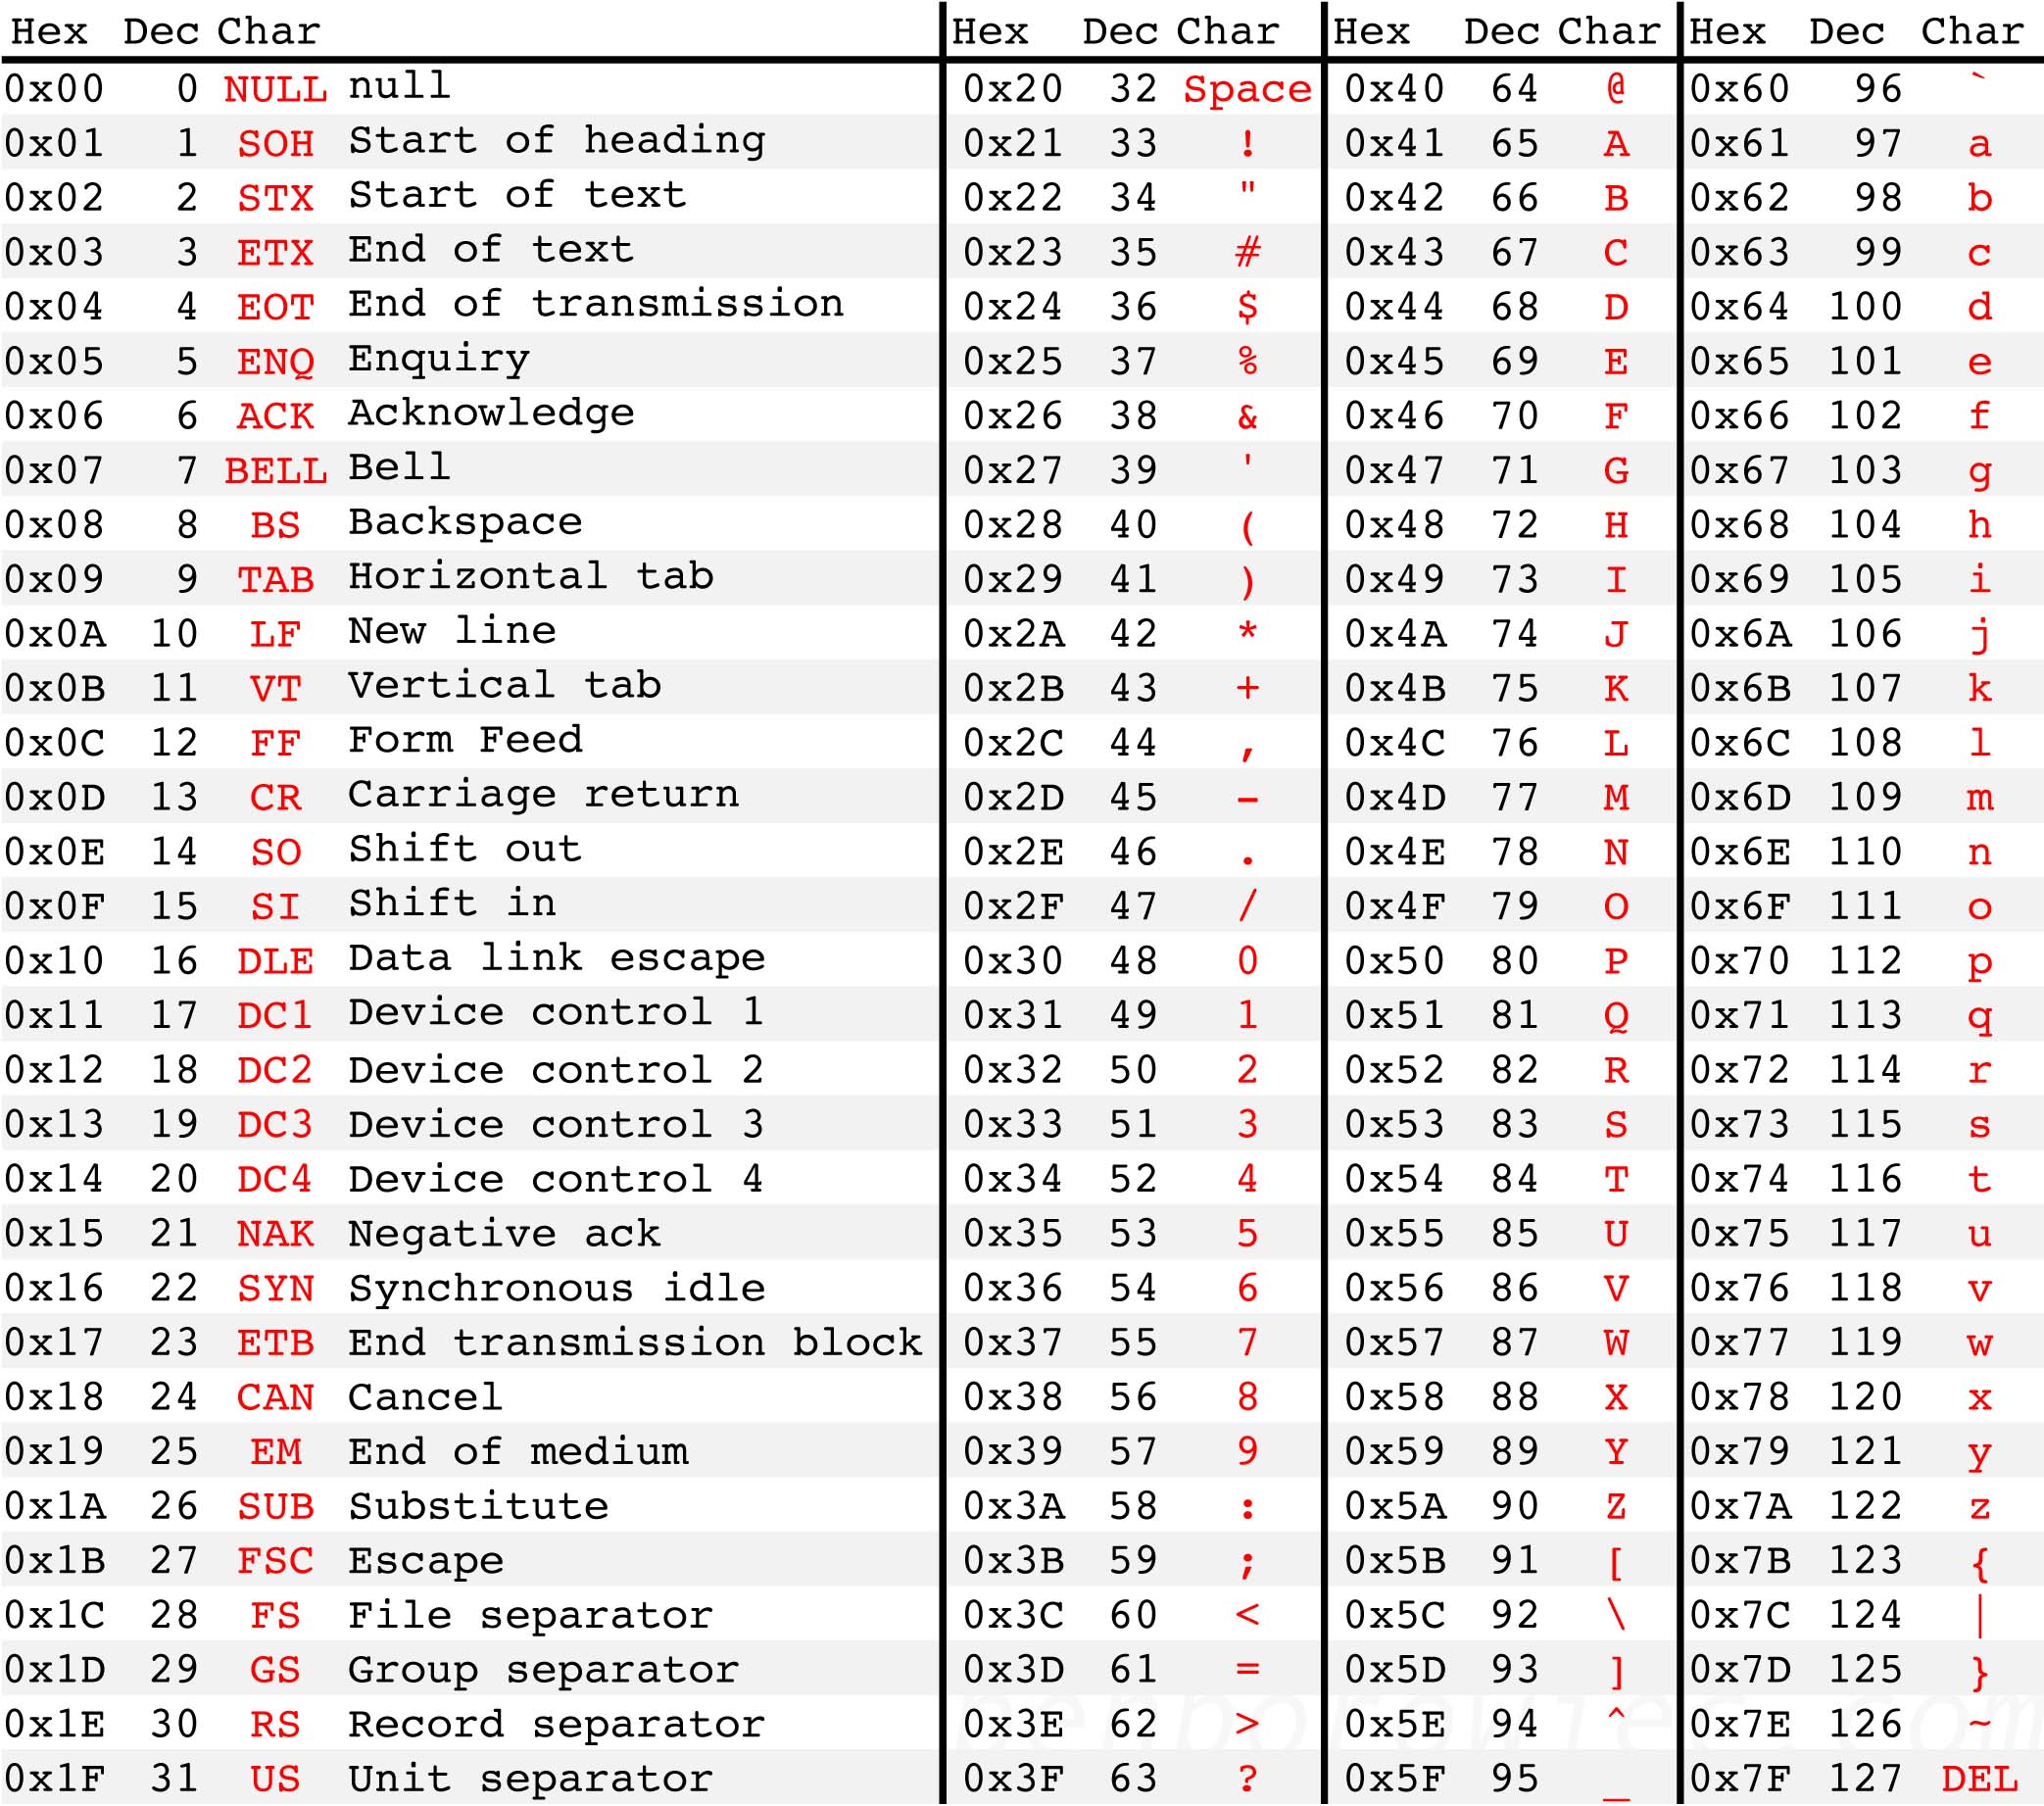
\includegraphics[width=.9\linewidth]{./img/ascii_table}
    \end{center}
\end{frame}

\begin{frame}{The Vastness of $\Sigma^*$}
    \begin{itemize}
        \item Suppose $\Sigma$ is the ASCII alphabet.
        \item Then what does $\Sigma^*$ contain?
    \end{itemize}

    \begin{center}
        \visible<2>{
        \huge\textcolor{SteelBlue4}{\bfseries Everything!}
        }
    \end{center}
\end{frame}

\begin{frame}{Elements of $\Sigma^*$}
    \begin{center}
        \begin{tikzpicture}
            \node[circle, thick,
                  draw=SteelBlue4, fill=SteelBlue4!25,
                  minimum size=10em,
                  font=\huge]
                (sigma) at (0,0) {$\mathbf{\Sigma^*}$};

            \node (shakespeare) [above right=.5em and 1em of sigma,
                                 visible on=<2->]
                {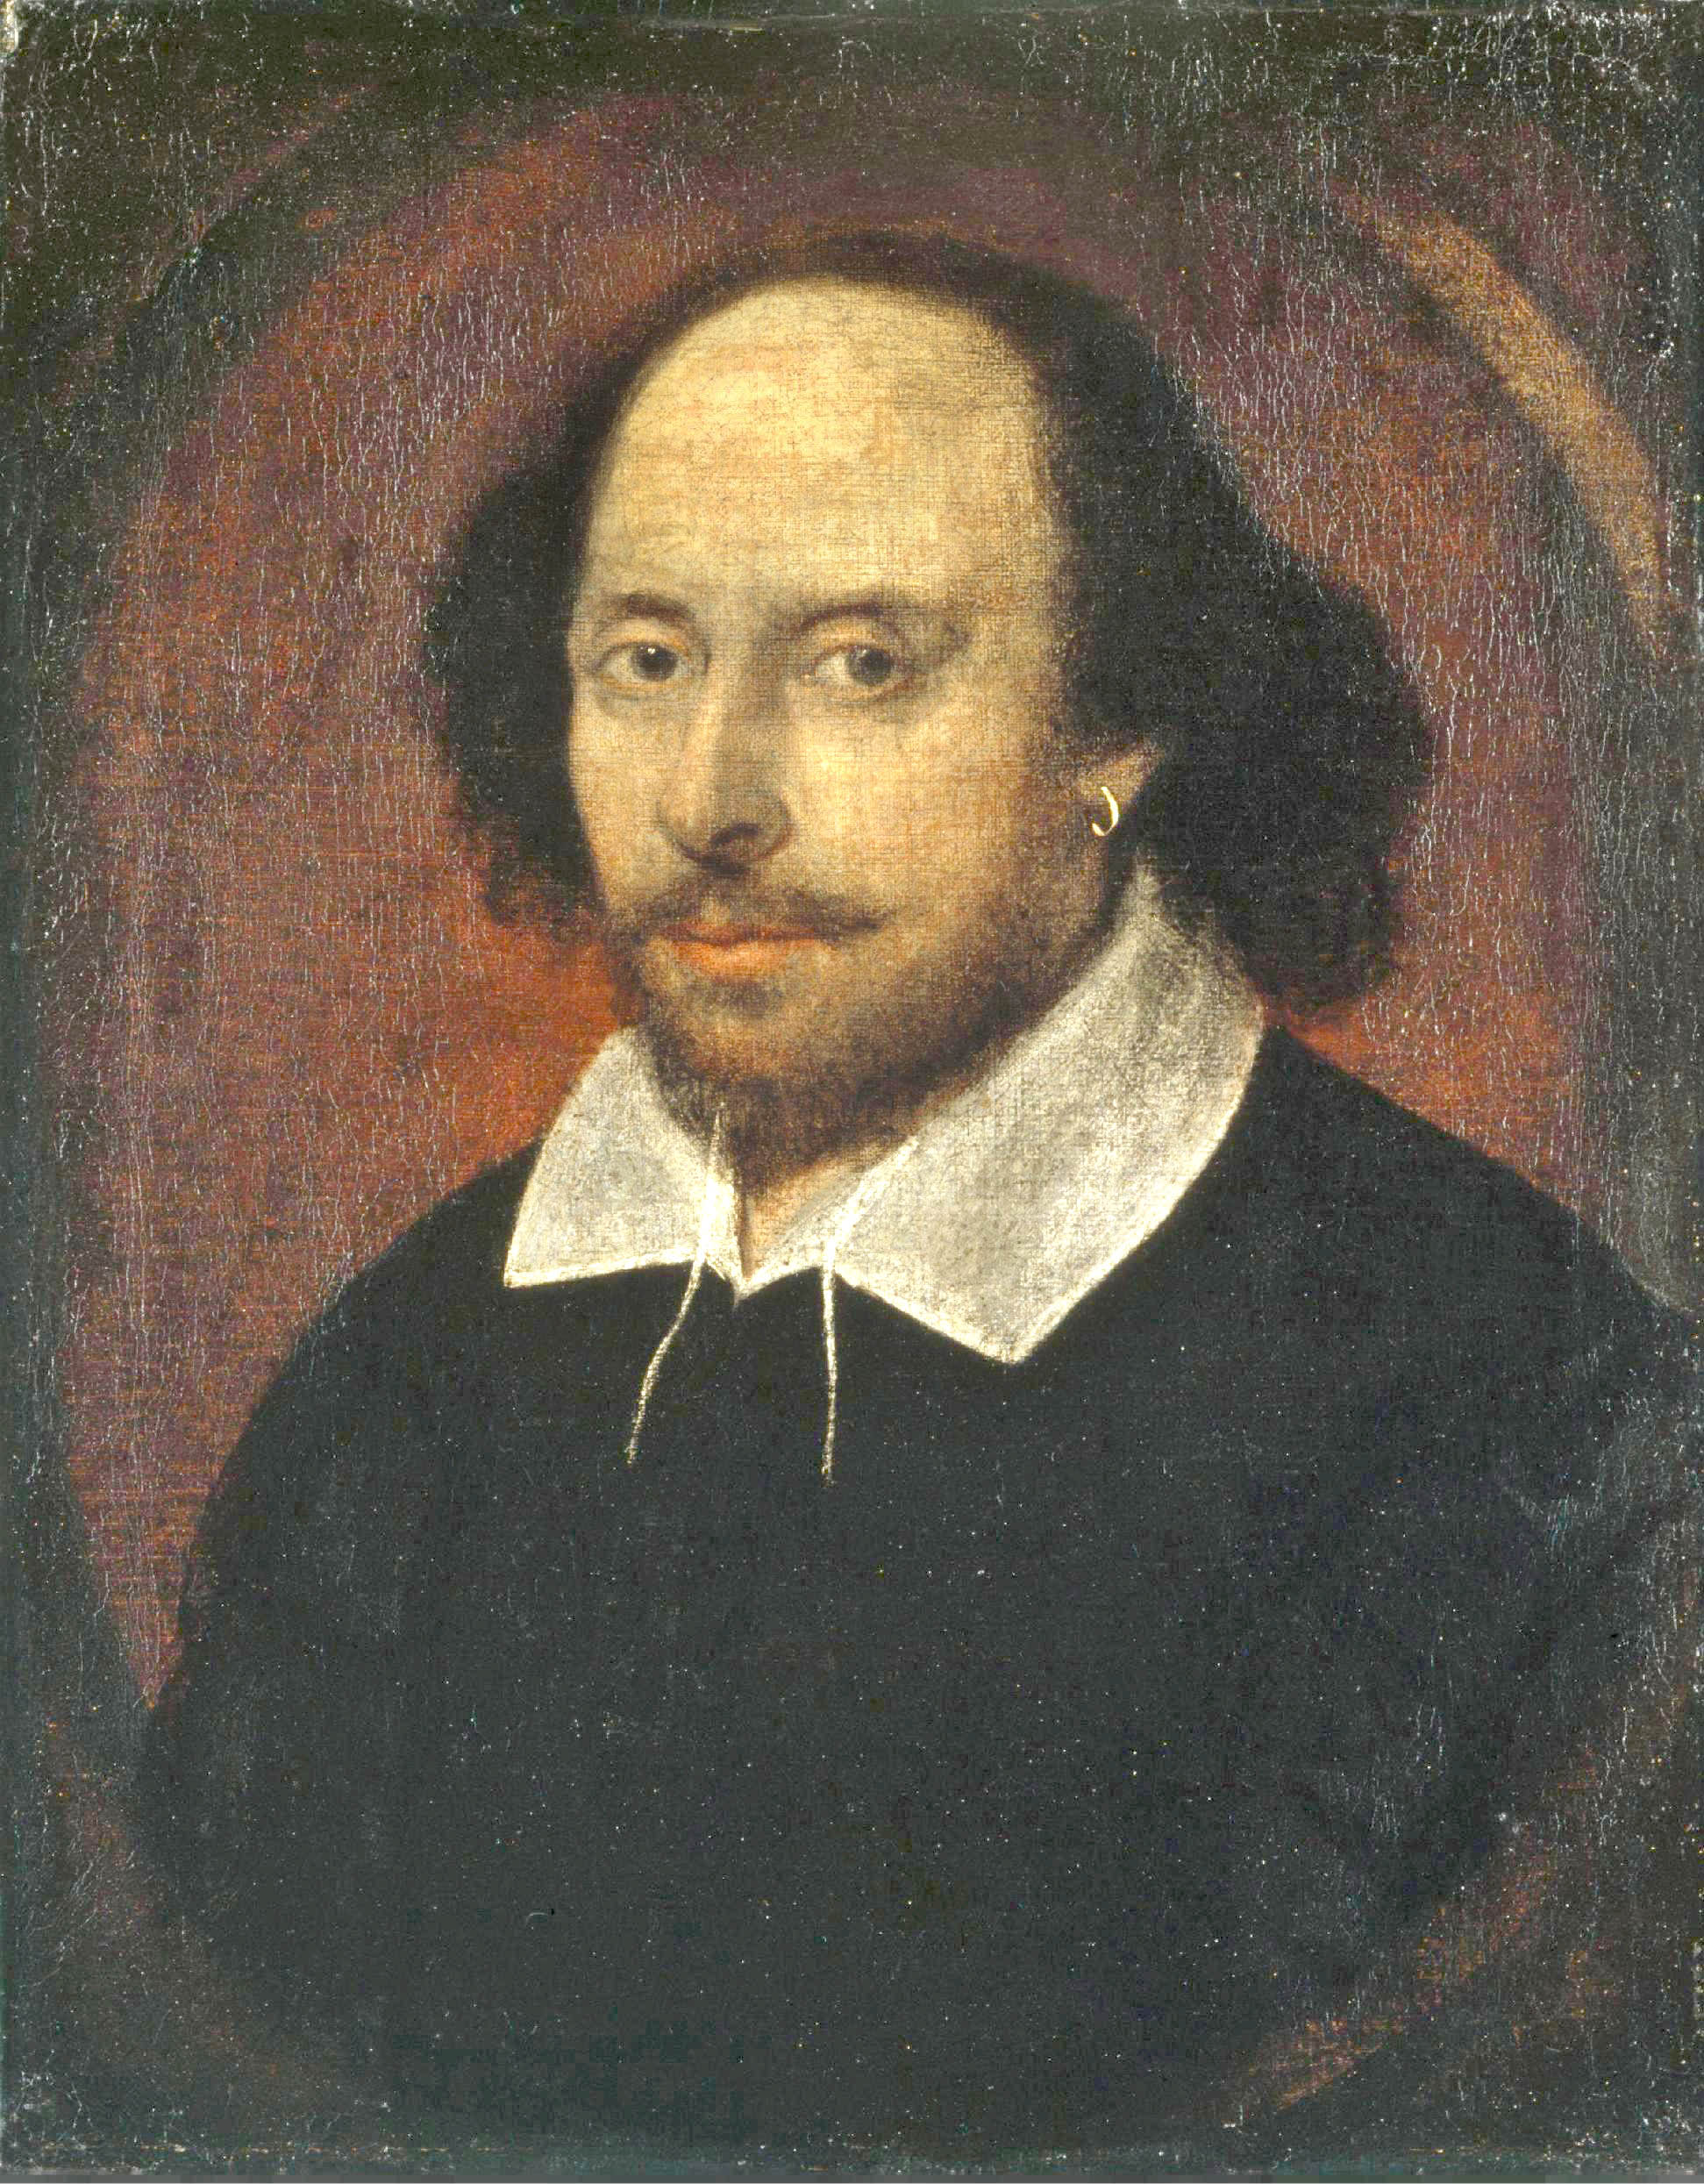
\includegraphics[width=6em]{./img/shakespeare}};

            \node (trump) [above left=1em and 1em of sigma,
                           visible on=<3->]
                {
\includegraphics[width=9em]{./img/trump}};

            \node (lotto) [below left=-1em and 2em of sigma,
                           visible on=<4->]
                {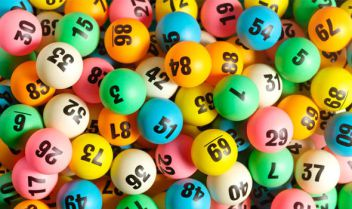
\includegraphics[width=9em]{./img/lotto}};

            \foreach \Source/\x/\y/\Counter in {%
                shakespeare/2/2/2,
                trump/-2/2/3,
                lotto/-2/-2/4}
                \draw[->, thick, purple,
                      decorate, decoration={snake, amplitude=.3em, post length=.75em},
                      visible on=<\Counter->]
                    (\Source) to ($(sigma.center)+(\x em, \y em)$);
        \end{tikzpicture}
    \end{center}
\end{frame}

\begin{frame}{$\Sigma^*$ has all the answers\ldots}
    $\Sigma^*$ contains everything that can be expressed\\
    with the chosen alphabet $\Sigma$.
    \begin{itemize}
        \item \textbf{ASCII}
            \begin{itemize}
                \item collected works of Shakespeare
                \item all tweets that Donald Trump deleted halfway through
                \item the funniest joke never told
                \item the list of your previous boy/girlfriends
            \end{itemize}
        \item \textbf{ASCII + mathematical symbols}
            \begin{itemize}
                \item all truths of mathematics
                \item all numbers that can be read as an English word (80085)
            \end{itemize}
        \item \textbf{cytosine, guanine, adenine, thymine}
            \begin{itemize}
                \item the genomes of all humans that were abducted by aliens
            \end{itemize}
    \end{itemize}
    It seems like $\Sigma^*$ is the key to \highlight{omniscience}.
\end{frame}

\begin{frame}[fragile]{And we can generate $\Sigma^*$\ldots}
    \begin{itemize}
        \item It is very easy to write a generator for $\Sigma^*$.
    \end{itemize}
\begin{pythoncode}
    # define some alphabet
    alphabet = [a, b, c, # and so on

    # add a special symbol, e.g. ß, to the alphabet
    # to separate distinct members of Sigma*
    list.append(alphabet, "ß")

    # then start generating indefinitely
    while True:
        print(random.choice(alphabet), end="")
\end{pythoncode}

\pause
\begin{exampleblock}{Example Output After Some Time}
\begin{pythoncode}
    "aas/ fk-j 23 819ßakerß555The answer to the next quiz isß/asd;k"
\end{pythoncode}
\end{exampleblock}

\pause
    \begin{itemize}
        \item Keep the code running forever, and it will produce everything that could ever be written, said, or thought.
    \end{itemize}
\end{frame}

\begin{frame}{The Proverbial Monkey on a Typewriter}
    \begin{itemize}
        \item \textbf{Problem}: our generator mostly produces gibberish
    \end{itemize}
    \begin{center}
        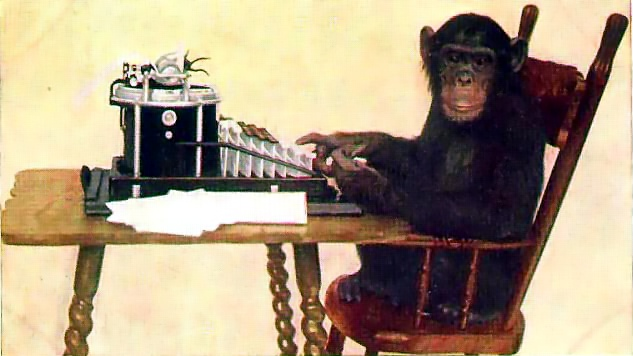
\includegraphics[width=.95\linewidth]{./img/monkey_typewriter}

    \end{center}
\end{frame}

\begin{frame}{The Moral of the Story}
    \begin{itemize}
        \item $\Sigma^*$ contains all truths.
        \item But the truth is drowned out among the noise.
        \item True knowledge is the ability to filter out the noise:
            \begin{enumerate}
                \item Know \highlight{what to look for}.
                \item Know \highlight{how to look for it}.
            \end{enumerate}
    \end{itemize}

    \begin{followup}
        \begin{itemize}
            \item Jorge Luis Borges' short story \emph{The Library of Babel}
            \item The library exists!\\
                  Try it online at \url{https://libraryofbabel.info/}
        \end{itemize}
    \end{followup}
\end{frame}

\begin{frame}{Back to Regular Expressions}
    \begin{itemize}
        \item What does all of this have to do with regular expressions?
        \item Regular expressions are our tool for getting rid of the noise.
        \item Just like $\Sigma^*$ is full of irrelevant noise,\\
              any given string may be full of irrelevant stuff. 
        \item With regular expressions, we can pick out the parts\\
            that we care about and forget about the rest.
    \end{itemize}
\end{frame}

\begin{frame}{Basic Building Blocks of Regular Expressions}
    The syntax of regular expressions varies slightly between implementations.
    We'll follow the Python conventions:

    \begin{center}
        \begin{tabular}{cl}
            \textbf{Pattern} & \textbf{Match}\\
            string & string\\
            . & any single character, including whitespace\\
            {\^{}} & beginning of line\\
            \$ & end of line\\
            $\lbrack$\colored{teal}{x},\colored{purple}{y}, \ldots] & characters \colored{teal}{x}, \colored{purple}{y}, \ldots\\
            $\lbrack$\colored{teal}{x}-\colored{purple}{y}] & all characters from \colored{teal}{x} to \colored{purple}{y}\\
            (\colored{teal}{x}$\ |\ $\colored{purple}{y}) & strings matching \colored{teal}{x} or \colored{purple}{y}\\
            \colored{teal}{x}$\{\colored{blue}{m}\}$ & exactly $\colored{blue}{m}$ instances of \colored{teal}{x}\\
            \colored{teal}{x}$\{\colored{blue}{m},\}$ & at least $\colored{blue}{m}$ instances of \colored{teal}{x}\\
            \colored{teal}{x}$\{,\colored{orange}{n}\}$ & at most $\colored{orange}{n}$ instances of \colored{teal}{x}\\
            \colored{teal}{x}$\{\colored{blue}{m},\colored{orange}{n}\}$ & between $\colored{blue}{m}$ and $\colored{orange}{n}$ instances of \colored{teal}{x}\\
            \colored{teal}{x}? & same as \colored{teal}{x}$\{\colored{blue}{0}, \colored{orange}{1}\}$ $\Rightarrow$ \colored{teal}{x} is optional\\
            \colored{teal}{x}$+$ & same as \colored{teal}{x}$\{\colored{blue}{1},\}$ $\Rightarrow$ one or more \colored{teal}{x}\\
            \colored{teal}{x}$*$ & same as \colored{teal}{x}$\{\colored{blue}{0},\}$ $\Rightarrow$ zero or more \colored{teal}{x}\\
        \end{tabular}
    \end{center}
\end{frame}

\begin{frame}{Examples of Regular Expressions} 
    Below are a few regexes, and for each regex
    some English words that match the described pattern.

    \small
    \begin{center}
        \begin{tabular}{ll}
            \textbf{Regex}                   & \textbf{Some Representative Matches}\\
            \texttt{test}                    & \visible<2->{test, testing, protests, vastest}\\
            \texttt{tes?t}                   & \visible<3->{test, testing, protests, vastest, untether}\\
            \texttt{tes?t?}                  & \visible<4->{test, testing, winter, zygotes, stethoscope}\\
            \texttt{t(es)?t}                 & \visible<5->{test, testing, vastest, wettest, better}\\
            \texttt{\^{}test}                & \visible<6->{test, testing, testify}\\
            \texttt{\^{}te+s?t}              & \visible<8->{test, testing, testify, teet}\\
            \texttt{\^{}.?t.*e+s?t}          & \visible<9->{test, testing, testify, teet, street, strangest}\\
            \texttt{\^{}.?t.*e+s?t\$}        & \visible<10->{test, teet, street, strangest}\\
            \texttt{\^{}te+[a-c].*s\$}       & \visible<11->{tea's, teachers, teazels, technocrats}\\
            \texttt{\^{}te+([a-c]|st?).*s\$} & \visible<12->{tests, testing, tea's, technocracts}\\
        \end{tabular}
    \end{center}
\end{frame}

\begin{frame}{So What are Regexes Good For?}
    \begin{itemize}
        \item Regular expressions are not specific to language technology.
            \begin{itemize}
                \item text search
                \item search and replace
                \item renaming files
                \item syntax highlighting for programmers (like in Jupyter notebook)
            \end{itemize}
        \item But they are part of tons of language technology:
        \begin{itemize}
            \item chatbots (see the homeworks)
            \item data analysis (discussed later in semester)
            \item simple grammar checker
        \end{itemize}
    \end{itemize}
\end{frame}

\begin{frame}[fragile]{Regexes for Grammar Checking}
    \begin{itemize}
        \item A \textbf{real-word error} is a spelling error where the word is spelled incorrectly given its context.
        \item Example: \emph{Their is a man in the garden}.
        \item can be detected with regular expressions
    \end{itemize}
    %
\begin{pythoncode}
    r"[Tt]heir (is|are|may|must|seems? )"
\end{pythoncode}
\end{frame}

\begin{frame}[fragile]{Another Grammar Checking Example}
    Number agreement between subject and verb:
    \begin{exe}
        \ex
        \begin{xlist}
            \ex[] {(All) (the) neighbors of Bill are always annoying.}
            \ex[*] {(All) (the) neighbors of Bill is always annoying.}
        \end{xlist}
    \end{exe}

    \noindent
    \textbf{Simplified Regex for Finding Agreement Error}
\begin{pythoncode}
    r"^(All )?[Tt]he [A-Za-z]+s( of [A-Za-z]+)? is"
\end{pythoncode}

    \begin{itemize}
        \item In practice, regexes are too clunky for\\
            fully adequate grammar checking.
        \item But regexes are part of many grammar checkers.
    \end{itemize}
\end{frame}

\begin{frame}[fragile]{Quick Break: Another Practice Session}
    For each regex, say whether \emph{Sue left...} is matched by it.

\pause
\begin{pythoncode}
    r"^s.+t"
\end{pythoncode}

\pause
\begin{pythoncode}
    r"^S.+t"
\end{pythoncode}

\pause
\begin{pythoncode}
    r"^S.+t$"
\end{pythoncode}

\pause
\begin{pythoncode}
    r"^S.+t\.$"
\end{pythoncode}

\pause
\begin{pythoncode}
    r"^S.+t\.*$"
\end{pythoncode}

\pause
\begin{pythoncode}
    r"^S.+(p|r|f).*t\.*$"
\end{pythoncode}

\visible<8>{
\begin{block}{Answers}
    1.~No\quad
    2.~No\quad
    3.~No\quad
    4.~No\quad
    5.~Yes\quad
    6.~Yes\quad
\end{block}
}
\end{frame}

\begin{frame}[fragile]{Additional Regex Tricks: Special Characters and Negation}
    \begin{itemize}
        \item A text may contain tabs and new lines, which we can't type directly in regexes.
        \item Instead, we have to use the special characters \texttt{$\backslash$t} and \texttt{$\backslash$n}.
    \end{itemize}
\begin{pythoncode}
    # match comma, semicolon or hyphen before a linebreak
    r"[,;-]\n"
\end{pythoncode}
    \begin{itemize}
        \item Sometimes, we want to say ``do \textbf{not} match x, y, or z''.
        \item This is written \texttt{[\^{}xyz]}.
    \end{itemize}
\begin{pythoncode}
    # match comma, semicolon or hyphen NOT before a linebreak
    r"[,;-][^\n]"
\end{pythoncode}
\end{frame}

\begin{frame}[fragile]{Additional Regex Tricks: Classes}
    We can already define lists of characters,\\
    but sometimes this can be cumbersome. 

\begin{pythoncode}
    # a regex for matching any word or variable name
    r"[A-Za-z0-9_]+"
\end{pythoncode}

    \highlight{Classes} are shorthands for specific lists.

    \begin{center}
        \begin{tabular}{cll}
            \textbf{Class} & \textbf{Equivalent to} & \textbf{Mnemonic}\\
            \texttt{$\backslash$w} & \texttt{[A-Za-z0-9\_]}                     & \textbf{w}ord\\
            \texttt{$\backslash$W} & \texttt{[\^{}A-Za-z0-9\_]}                 & \textbf{NOT} \textbf{w}ord\\
            \texttt{$\backslash$d} & \texttt{[0-9]}                             & \textbf{d}igit\\
            \texttt{$\backslash$D} & \texttt{[\^{}0-9]}                         & \textbf{NOT} \textbf{d}igit\\
            \texttt{$\backslash$s} & \texttt{[ $\backslash$t$\backslash$n]}     & white\textbf{s}pace\\
            \texttt{$\backslash$S} & \texttt{[\^{} $\backslash$t$\backslash$n]} & \textbf{NOT} white\textbf{s}pace\\
        \end{tabular}
    \end{center}
\end{frame}

\begin{frame}[fragile]{Some Examples}
\begin{enumerate}
    \item Matching all words, and nothing else\\
        (this will be really important for us in the next lecture)
\begin{pythoncode}
    r"\w+"
\end{pythoncode}
    \item Matching all AD years
\begin{pythoncode}
    r"\d{1,4}"
\end{pythoncode}
    \item Finding two words with arbitrary amount of whitespace between them
\begin{pythoncode}
    r"\w+\s+\w+"
\end{pythoncode}
\end{enumerate}
\end{frame}

\begin{frame}[fragile]{The Final Trick: Backreferences}
    \begin{itemize}
        \item The brackets \texttt{(} and \texttt{)} also define groups.
        \item For example, the \textbf{backreference} \texttt{$\backslash$2} refers to the 2nd group.
    \end{itemize}

\begin{pythoncode}
    # convert dates from month/day/full_year to full_year-month-day
    re.sub(r"(\w+)/(\d{,2})/(\d{4})",
           r"\3-\1-\2",
           string)
\end{pythoncode}

    \begin{itemize}
        \item Backreferences allow chatbots to reuse parts of the user input.
    \end{itemize}
\end{frame}

\begin{frame}{Tips for Reading and Writing Regular Expressions}
    \begin{itemize}
        \item \textbf{Practice, practice, practice!}\\
            Regular expressions take a while to get used to.
            Practice on
            \begin{itemize}
                \item Pythex: \url{https://pythex.org}
                \item RegexOne: \url{https://regexone.com/lesson/introduction_abcs}
            \end{itemize}
        \item \textbf{Don't panic!}\\
            Regexes look confusing, but just work your way trough them left-to-right and you'll soon know what's going on.
        \item \textbf{It's the patterns, stupid!}\\
            If you want to clean up a string with regexes, think about what exactly the pattern is that you're trying to extract.
            If you can phrase it as something like ``all the stuff between the first vowel and the third consonant'', you are already halfway done with your regex.
    \end{itemize}
\end{frame}

\begin{frame}{Summary}
    \begin{itemize}
        \item Regular expressions are an essential for pattern matching.
            \begin{itemize}
                \item clean up data
                \item modify and recycle user input
                \item grammar checking
                \item and much more
            \end{itemize}
        \item At this point they will still feel strange to you, but by the end of the semester
              you'll be fairly comfortable with them.
    \end{itemize}
\end{frame}

% \begin{frame}[fragile]{So What was That Weird Regex About?}
%     Remember this guy?
%
% \begin{pythoncode}
%     re.sub(r'^.*?id="(\w+)".*?<h3>.*?:\s*(.*?)</h3>.*?<p>(.*?)</p>(.*)',
%            r"\1|\2|\3|\4",
%            course_description)
% \end{pythoncode}
%
%     Now that we know a bit about regular expressions,\\
%     let's go through it step by step.
% \end{frame}
%
% \begin{frame}[fragile]{Step 1: Eye-Balling the Files}
%     \begin{itemize}
%         \item After running some code to download all the relevant pages,\\
%             I looked at some of the files to get a feeling for the data.
%         \item Each file is an HTML file with the descriptions for all courses in a program.
%             Here's an excerpt:
%     \end{itemize}
%
% {\small
% \begin{minted}{HTML}
% <div class="course" id="120">
%     <h3>LIN 120: Language and Technology</h3>
%     <p>An introduction to how computers process language.</p>
%     <span style="font-style: italic">SBC:</span>
%     <a title="Understand Technology">TECH</a>
%     <p>3 credits</p>
%     <div class="clear"></div>
% </div>
% <div class="course" id="200">
%     <h3>LIN 200: Language in the United States</h3>
% \end{minted}
% }
% \end{frame}
%
% \begin{frame}[fragile]{Step 2: Extracting the Full Course Descriptions}
%     \begin{itemize}
%         \item Each course description starts with \mintinline{HTML}{<div class="course"} and then continues until \mintinline{HTML}{<div class="clear">}.
%         \item We will use a regular expression to split the file into a list of course descriptions.
%     \end{itemize}
%
% \begin{pythoncode}
%     courses = re.findall(r'<div class="course".*?<div class="clear"')
% \end{pythoncode}
% \end{frame}
\end{document}
